
\chapter{Stochastic Hamiltonian systems}\label{ch:the_diffusive_framework}

After having introduced the basic concepts of the theory of stochastic Hamiltonian systems in Chapter~\ref{ch:mathematical_elements}, we now turn to the study of the diffusive properties of these systems. These properties are related to the introduction of a stochastic perturbation in the Hamiltonian of the system.

We will first present the general framework of the theory of stochastic Hamiltonian systems, inspecting some simple examples of diffusion over toroidal surfaces. Next, we will focus on the application of the averaging principle on stochastic Hamiltonian systems, and show how it is possible to reach an expression of the diffusion process of the system in terms of a Fokker-Planck equation, whose diffusion coefficient $D(I)$ has a functional form related to the Nekhoroshev theorem.

\section{Stochastic perturbations}

\subsection{Diffusion over a toroidal surface}
\label{subsec:Diffusion for a stochastically perturbed integrable system}

We start by investigating the fast diffusion process of a probability distribution over a toroidal surface. We are interested in this process as such situation occurs in action-angle Hamiltonian systems for the angle variable.

Let us start by defining the following notation: if $\xi(s)$ is a regular stationary stochastic Gaussian process, we set:
\begin{equation}
	w(t) = \int_0^t \xi(s)\,\mathrm{d}s \,, \qquad w_1(t)=\int_0^t w(t)\,\mathrm{d}s \,,
\end{equation}
The realisations $\xi(t)$ are continuous, with a correlation function 
\begin{equation}
    \langle\xi(t)\xi(t+\tau)\rangle = \Omega(\gamma\tau) \,,\qquad \Omega(\gamma\tau) \simeq \frac{\gamma}{2}e^{-\gamma|\tau|}\,.
\end{equation}
The limit $\gamma\to\infty$ is the white noise limit where the process $\xi(t)$ looses its regularity. Then $w(t)$ is the Wiener process. We can write \(w_1(t)\) in the form
\begin{equation}
	w_1(t) = \int_0^t \int_0^s \xi(u)\,\mathrm{d}u\,\mathrm{d}s' = \int_0^t \xi(u)\int_u^s\,\mathrm{d}s'\,\mathrm{d}u = \int_0^t (s'-u)\xi(u)\,\mathrm{d}u \,.
\end{equation}
This form is convenient if we want to present the processes \(w(t)\) and \(w_1(s)\) in the standard form 
\begin{equation}
	\int_0^t K(t,s)\xi(s)\,\mathrm{d}s \,
\end{equation}
where \(K(t,s)\) is called the \textit{kernel} of the noise. We have that \(K=1\) for \(w(t)\) and \(K=t-s\) for \(w_1(t)\). This implies that the variance is \(\sigma^2(t) = t\) for Wiener noise \(w(t)\) while for its integral \(w_1(t)\), we have
\begin{equation}
	\sigma^2(t) = \int_0^t (t-u)^2\,\mathrm{d}u = \frac{t^3}{3} \,.
\end{equation}

Let us consider a simple example of angular diffusion. Let \(x\) be an angular variable defined over the interval \([0,1]\). We consider the stochastic Hamiltonian dynamics
\begin{equation}
	\begin{aligned}
		\dot{\phi} &= \omega + I \mod{1}\,, \\
		\dot{I} &= \epsilon\xi(t)	\,.
	\end{aligned}
	\label{eq:langevin_toro}
\end{equation}
The distribution function \(\rho_T(\hat{x},t)\) for the angular variables\(\hat{\phi}\) can be defined using the solution  \(\rho(\hat{x},t)\) with open boundary conditions on \(\mathbb{R}\) using
\begin{equation}
	\rho_T(x,t) = \sum_{k=-\infty}^{+\infty} \rho(x+k,t) \quad x\in[0,1]\,,\quad k = 0,\pm 1, \pm 2, \ldots \,.
 \label{eq:period}
\end{equation}

In the white noise limit the solution of~\eqref{eq:langevin_toro} on \(\mathbb{R}\) is given by
\begin{equation}
	y = y_0 + \epsilon w(t)\,, \qquad x = x_0 + (\omega + \epsilon y_0) t + \epsilon w_1(t) \,,
\end{equation}
by writing the evolution of the average value of \(x(t)\) in the form \(\langle x(t) \rangle = x_0 + (\omega + \epsilon y_0) t\), $x(t)$ is a Gaussian process and the probability density in \(\mathbb{R}\) reads
\begin{equation}
	\rho(x,t) = \frac{\exp{\frac{-(x-\langle x(t)\rangle)^2}{2\sigma^2(t)}}}{\sqrt{2\pi\sigma^2}}\,, \qquad \sigma^2(t) = \epsilon^2 \frac{t^3}{3}\,,
\end{equation}
we can then apply~\eqref{eq:period} and finally obtain
\begin{equation}
	\rho_T(x,t) = \sum_{n=-\infty}^{+\infty} \frac{\exp{\frac{-(x-\langle x(t)\rangle + n)^2}{2\sigma^2}}}{\sqrt{2\pi\sigma^2}} \,\qquad n = 0,\pm 1, \pm 2, \ldots\,.
\end{equation}

If we represent the solution in the form of a Fourier series,
\begin{equation}
	\rho_T(x,t) = \sum_{k=-\infty}^{+\infty} f_k(t)e^{2\pi i k x} \,,
\end{equation}
the \(f_k\) coefficients are given by
\begin{align}
	f_k &= \int_0^1 e^{-2\pi i k x} \rho_T(x,t)\,\mathrm{d}x \\
	&= \sum_{n=-\infty}^{+\infty} \frac{1}{\sqrt{2\pi\sigma^2}} \int_0^1 \exp{\frac{-(x-\langle x(t) \rangle + n)^2}{2\sigma^2} -2\pi i k x}\,\mathrm{d}x \,.
\end{align}
By assuming real \(f_k\) coefficients, we obtain
\begin{equation}
	\rho_T(x,t) = 1+2\sum_{k=1}^\infty e^{-2\pi^2\sigma^2k^2} f_k \cos(2\pi k (x-\langle x(t) \rangle)) \,.
\end{equation}

The most important aspect of this example, is how \(\rho_T\) relaxes to the uniform distribution \(\propto e^{-\sigma^2(t)}\), and the relaxation time scale can be estimated by
\begin{equation}
	\sigma^2 \propto \epsilon^2 t^{3}\simeq 1 \,,
\end{equation}
so that $t\simeq \epsilon^{-2/3}$,
while for the Wiener process $y(t)$ the diffusion time scale is $t\simeq \epsilon^{-2}$ since
\begin{equation}
	\sigma^2 \propto t \,.
\end{equation}

\subsubsection*{Application to integrable Hamiltonian systems}

Let us consider the following perturbed Hamiltonian system
\begin{equation}
	\ham = \ham_0(I) - \epsilon \phi \xi(t)\,.
\end{equation}
From this Hamiltonian, we have the equations of motion
\begin{equation}
	\begin{aligned}
		{I'} &= \epsilon\xi\,, \\
		{\phi'} &= \omega(I)\,,
	\end{aligned}
\end{equation}
from which follows immediately
\begin{equation}
	I = I_0 + \epsilon w(t)\,.
\end{equation}
Therefore the action is a Gaussian process with average value $I_0$ and variance
\begin{equation}
	\sigma_{I}^2=\epsilon^2t\,.
\end{equation}
In a perturbation approach $\epsilon\ll 1$ we study the evolution of the system for a time $t\ll \epsilon^{-2}$. Then in the  Taylor expansion for \({\phi'}\), we obtain
\begin{equation}
	{\phi'} = \omega(I_0) + \omega'(I_0)\epsilon w(t) + \mathcal{O}(\epsilon^2)\,,
\end{equation}
the contribution of the term $\mathcal{O}(\epsilon^2)$ can be neglected at this time scale. A direct integration leads to
\begin{equation}
	\phi = \phi_0 + \omega(I_0)t + \epsilon \omega'(I_0) w_1(t)\,.
\end{equation}
so that the relaxation time scale of the angle variable is estimated by
\begin{equation}
	\sigma_{\phi}^2 \propto \epsilon^2 t_\phi^3\simeq 1
\end{equation}
i.e. $t_\phi\simeq \epsilon^{-2/3}$. The perturbation approach is justified if one chooses $t\simeq t_\phi$ since $t\epsilon^2\simeq \epsilon^{4/3}\ll 1$. It follows that the angle variable can be considered a fast variable in the diffusion process whereas the action is a slow variable.

\subsection{Averaging a 1\textsc{d} stochastic Hamiltonian}
\label{ssc:averaging-1D}

Let us consider a generic 1\textsc{d} stochastically perturbed Hamiltonian system in action-angle coordinates,
\begin{equation}
	\ham = \ham_0(I) + \epsilon \xi(t) \ham_1(\phi, I) \,.
\end{equation}
We remark that the symplecticity character of the phase solving the canonical equation requires that the stochastic process $\xi(t)$ has continuous realizations. In such a case the white noise limit can be performed by considering the average solution of the stochastic Liouville equation
\begin{equation}
	\pdv{\rho}{t}\/ + \Omega \pdv{\rho}{\phi}\/ +\epsilon \xi(t)\{\ham_1,\rho\}=0
\end{equation}

where \(\{\ ,\}\) are the Poisson brackets and \(\Omega(I) = \partial \ham_0/\partial I\).
In the white noise limit one can proves that The probability density \(\rho(\phi, I; t)\)  satisfies the Fokker-Planck equation
\begin{equation}
	\pdv{\rho}{t}\/ + \Omega \pdv{\rho}{\phi}\/ = \frac{\epsilon^2 \sigma^2}{2}\{\ham_1, \{\ham_1,\rho\}\}
	\label{eq:stoc_ham_complex_starting}
\end{equation}
that corresponds to the Stratonovich interpretation of the stochastic canonical equations. In the diffusion limit $\epsilon\to 0$ and $t\gg 1$ with
$t\epsilon^2=O(1)\gg t_{\phi}$ according to the results of the previous section, it is possible to apply an averaging theorem to the angle variable dynamics. This allows us to simplify this last equation into a Fokker-Planck equation, which describes the evolution of the distribution for the action variable \(\rho(I,t)\)
\begin{equation}
	\pdv{}{t}\/\rho(I,t) = \pdv{}{I}\/D(I)\pdv{}{I}\/\rho(I,t) \,,
\end{equation}
where
\begin{equation}
	D(I) = \frac{\epsilon^2 \sigma^2}{2}\frac{1}{2\pi}\int_0^{2\pi}\left(\pdv{\ham_1}{\phi}\/\right)^2 \,d\phi \equiv \frac{\epsilon^2 \sigma^2}{2} \left\langle \left( \pdv{\ham_1}{\phi}\/  \right)^2 \right\rangle_\phi \,.
\end{equation}

\subsubsection*{Proof}
Let us start from the stochastic Liouville equation
\begin{equation}
	\pdv{\rho}{t}\/ + \Omega(I) \pdv{\rho}{\phi}\/ + \epsilon\xi(t)\{\rho,\ham_1\} = 0\,,
	\label{eq:dimo_liouville}
\end{equation}
from this, we can write \(\rho\) in the form \(\rho = \rho_0 + \epsilon\rho_1\), where \(\rho_0\) is the average component of the distribution and \(\rho_1\) the fluctuating component with zero mean. Considering that \(\langle\xi\rangle = 0\), we find that the average value of Eq.~\eqref{eq:dimo_liouville} can be written as
\begin{equation}
	\pdv{\rho_0}{t}\/ + \Omega(I)\pdv{\rho_0}{\phi}\/ + \epsilon^2\{\langle\xi(t)\rho_1\rangle, \ham_1\} = 0,.
	\label{eq:dimo_media}
\end{equation}
If we now subtract~\eqref{eq:dimo_media} from~\eqref{eq:dimo_liouville}, we obtain the equation
\begin{equation}
	%TODO: check this passages again (never trust past Carlo too much...)
	\pdv{\rho_1}{t}\/ + \Omega(I) \pdv{\rho_1}{\phi}\/ = -\xi(t)\{\rho_0, \ham_1\} + O(\epsilon)\,
\end{equation}
which we now want to solve for \(\rho_1\), and substitute it into Eq.~\eqref{eq:dimo_media}.

To archive this, let us consider the following change of variables:
\begin{equation}
	\begin{aligned}
		\phi &\to \phi - \Omega \tau\,, \\
		t &\to t - \tau\,.
	\end{aligned}		
\end{equation}
This change of variables allows us to group the last equation in the form
\begin{equation}
	\dv{}{\tau}\/\rho_1(\phi - \Omega \tau, I; t - \tau) = \xi(t- \tau)\{\rho_0, \ham_1\}(\phi - \Omega \tau, I; t - \tau)\,.
\end{equation}
If we now integrate this last equation from \(\tau = 0\) to \(\tau = t\), we obtain the following expression
\begin{equation}
	\rho_1(\phi, I, t) = -\int_0^t\{\rho_0, \ham_1\}(\phi - \Omega \tau, I, t - \tau)\xi(t-\tau)\,\mathrm{d}\tau\,,
\end{equation}
where we took advantage of the fact that \(\rho_1(\phi, I; 0)=0\). If we now multiply both members by \(\xi(t)\), and compute the average over all noise realisations, we have, for the case of a Wiener noise:
\begin{equation}
	\langle \xi(t)\rho_1(\phi, I; t) \rangle = -\frac{1}{2}\sigma^2 \{\rho_0, \ham_1\}(\phi, I; t)\,.
\end{equation}

Finally, if we insert this last result into Eq.~\eqref{eq:dimo_media}, we obtain, neglecting terms of order \(\epsilon^3\) or higher, the equation for the average density
\begin{equation}
 	\pdv{\rho_0}{t}\/ + \Omega (I) \pdv{\rho_0}{\phi}\/ = \frac{\epsilon^2 \sigma^2}{2}\{\{\rho_0, \ham_0\}, \ham_0\}.
\end{equation}

If we see that the relaxation timescale of the angle is faster than the diffusion timescale of the action, we can say, with good approximation, that \(\rho=\rho(I,t)\) does not depend on the angle variable \(\phi\). With this motivation, we can expand the double Poisson bracket expression, which reads
\begin{equation}
	\{\{\rho_0, \ham_0\}, \ham_0\} = \pdv{}{I}\/\left[\left(\pdv{\ham_1}{\phi}\/\right)^2 \pdv{\rho_0}{I}\/\right] - \pdv{}{\phi}\/\left[\pdv{\rho_0}{I}\/\pdv{\ham_1}{\phi}\/\pdv{\ham_1}{I}\/\right]\,,
\end{equation}
and take the angular average of this last equation. The second term in the r.h.s\ will then become zero, while the first term constitutes the expression of \(D(I)\), which now has to be integrated over the whole torus.

\subsection{Averaging principle for generic stochastic Hamiltonians}

We now generalise this last result to stochastically-perturbed Hamiltonian systems with higher dimensions. Let us start by considering a generic Hamiltonian system
\begin{equation}
	\ham = \ham_0(I) + \xi(t)\ham_1(\phi, I)\,,
\end{equation}
where \((\phi, I)\) are now, respectively, variables in $\mathbb{T}^n$ and $\mathbb{R}^n$ with $n>1$, and the noise realisation \(\xi(t)\) depends on the initial condition of the orbit.

We now introduce the slow variable
\begin{equation}
	\phi = \phi - \Omega(I)t\,,
\end{equation}
where \(\Omega(I) = \frac{\partial \ham_0}{\partial I}(I)\). This leads us to the new Hamiltonian
\begin{equation}
	\ham = \xi(t)\ham_1(\phi+\Omega(I)t,I)\,,
\end{equation}
via the generating function
\begin{equation}
	F(\phi,I) = \phi I - \ham_0(I)t\,.
\end{equation}

To find an approximate solution of the stochastic dynamic, we can consider the evolution of the action-angle variables for a time \(T\gg \lambda\). From the new Hamiltonian we now have
\begin{equation}
	\begin{aligned}
		\Delta\phi_j(T) &= \int_0^T\pdv{\ham_1}{I_j}\/(\phi+\Omega(I)t, I)\xi(t)\,\mathrm{d}t -\\
		&\qquad - \int_0^T t\pdv{\ham_1}{\phi_k}\/(\phi + \Omega(I)t,I)\pdv{\Omega_k}{I_j}\xi(t)\,\mathrm{d}t\\ \,,
		\Delta I_j(T) &= -\int_0^T\pdv{\ham_1}{\phi_j}\/(\phi+\Omega(I)t,I)\xi(t)\,\mathrm{d}t\,,
	\end{aligned}
	\label{eq:averaging-generic-hams}
\end{equation}
where \(\Delta \phi_j(T)=\phi(T)-\phi(0)\) and \(\Delta I(T)=I(T)-I(0)\).

We now focus our attention on the second integral in the expression of \(\Delta\phi_j(T)\). By performing an integration by parts, where we also truncate the expansion to higher orders, we reach the expression
\begin{multline}
	\int_0^T t\pdv{\ham_1}{\phi_k}\/(\phi+\Omega(I)t,I)\pdv{\Omega_k}{I_j}\xi(t)\,\mathrm{d}t \simeq \\
	\simeq \pdv{\Omega_k}{I_j}\/\bigg[T\int_0^T\pdv{\ham_1}{\phi_k}\/(\phi+\Omega(I)t,I)\xi(t)\,\mathrm{d}t\, - \\
	- \int_0^T\int_0^t\pdv{\ham_1}{\phi_j}\/(\phi+\Omega(I)s, I)\xi(s)\,\mathrm{d}s\,\mathrm{d}t\bigg]\,,
\end{multline}
from this, we can combine the resulting two integrals together and replace their arguments using the expression for $\Delta I_j(T)$ given in Eq.~\eqref{eq:averaging-generic-hams}, and obtain
\begin{equation}
	\int_0^T t\pdv{\ham_1}{\phi_k}\/(\phi+\Omega(I)t,I)\pdv{\Omega_k}{I_j}\xi(t)\,\mathrm{d}t \simeq \pdv{\Omega_k}{I_j}\int_0^T[\Delta I_k(T)-\Delta I_k(t)]\,\mathrm{d}t\,.
\end{equation}
This implies that if the action dynamics can be considered a stationary process, the main contribution to the angular dynamics is given by
\begin{equation}
	\Delta \phi_j \simeq -\pdv{\Omega_k}{I_j}\int_0^T\Delta I_k(t)\,\mathrm{d}t\,.
\end{equation}

If the system is non-degenerate, % i.e.\ the matrix \(\partial\Omega_k/\partial I_j\) is not singular,
the increment of $\phi$ is the integral of the increments of $I$ and, as illustrated above in this chapter, we expect consequently a faster relaxation to a uniform distribution. From these considerations we find that, when considering the evolution of $I$, we can approximate the $\phi$ distribution with a uniform one. If we now expand the expression of $\Delta I_j$ up to terms of order \(\mathcal{O}(\norm{\ham_1}^2)\), we obtain the following:
\begin{multline}
	\Delta I_j = \int_0^T \pdv{\ham_1}{\phi_j}\xi(s)\,\mathrm{d}s + \int_0^T\int_0^t \pdv{\ham_1}{I_k}{\phi_j}\pdv{\ham_1}{\phi_k}\xi(t)\xi(s)\,\mathrm{d}s\,\mathrm{d}t - \\
	- \int_0^T\int_0^t\pdv{\ham_1}{\phi_k}{\phi_j}\left[\pdv{\ham_1}{I_k}-\pdv{\Omega}{I_k}\pdv{\ham_1}{\phi_k}t\right]\xi(t)\xi(s)\,\mathrm{d}s\,\mathrm{d}t\,.
\end{multline}

If then we assume that the distribution of \(\phi\) is uniform, we can average on both the noise realizations and on $\phi$. We can then consider the average of the stochastic dynamics of \(I\), which now reads
\begin{equation}
	\begin{aligned}
		\langle\Delta I_j\rangle_\phi &= \pdv{}{I_k}\int_0^T\int_0^t \left\langle\pdv{\ham_1}{\phi_j}\pdv{\ham_1}{\phi_k}\right\rangle e^{-(t-s)/\lambda}\,\mathrm{d}s\,\mathrm{d}t\\
		&= \frac{1}{2}\pdv{}{I_k}\left\langle\pdv{\ham_1}{\phi_j}\pdv{\ham_1}{\phi_k}\right\rangle\int_0^T\int_0^T e^{-\abs{t-s}/\lambda}\,\mathrm{d}s\,\mathrm{d}t\,,
	\end{aligned}
\end{equation}
where we have neglected the terms that are pure derivatives of $\phi$, and considered the mean and decorrelation properties of \(\xi(t)\). The corresponding variance is then estimated by
\begin{multline}
	\left\langle(\Delta I_j - \langle\Delta I_j\rangle_\phi)(\Delta I_k - \langle\Delta I_k\rangle_\phi)\right\rangle_\phi =\\
	= \left\langle\pdv{\ham_1}{\phi_j}\pdv{\ham_1}{\phi_k}\right\rangle\int_0^T\int_0^T e^{-\abs{t-s}/\lambda}\,\mathrm{d}s\,\mathrm{d}t\,.
\end{multline}

We can then describe the action dynamics as a stochastic process of the form
\begin{equation}
	\Delta I_j = -\sqrt{T\lambda\norm{\ham_1}^2}\sqrt{\left\langle\pdv{\hat\ham_1}{\phi_j}\pdv{\hat\ham_1}{\phi_l}\right\rangle}\,\hat{\xi}_l + \frac{T\lambda\norm{\ham_1}^2}{2}\pdv{}{I_k}\left\langle\pdv{\hat\ham_1}{\phi_j}\pdv{\hat\ham_1}{\phi_k}\right\rangle\,
	\label{eq:generic-ham-average-almost}
\end{equation}
where \(\hat{\ham_1}=\ham_1/\norm{\ham_1}\) and \(\hat{\xi}_l\) are identical independent distributed random variables with zero mean value and unit variance. We can interpret the quantity \(T\lambda\norm{\ham_1}^2\) as the time step \(\Delta\tau\) of the diffusion time, we highlight, however, that it has a dimension of an action. Consequently, we then require that \(T\) should be sufficiently long in order to consider angles relaxing to a uniform distribution and noise decorrelated, but \(\norm{\ham_1}^2\) has to be so small that actions do not evolve in a time \(T\). 

If these conditions are maintained, introducing the notation \(\tau = \lambda\norm{\ham_1}^2 t\), we have that Eq.~\eqref{eq:generic-ham-average-almost} is the approximation of the solution of the stochastic differential equation
\begin{equation}
	\mathrm{d}I_j = -\sqrt{\left\langle\pdv{\hat\ham_1}{\phi_j}\pdv{\hat\ham_1}{\phi_l}\right\rangle}\,\mathrm{d}\omega_l(\tau) + \frac{1}{2}\pdv{}{I_k}\left\langle\pdv{\hat\ham_1}{\phi_j}\pdv{\hat\ham_1}{\phi_k}\right\rangle\,\mathrm{d}\tau\,.
	\label{eq:final-ham-approximation}
\end{equation}

% In order to completely check the consistency of our claims, let us consider again the angle dynamics in the diffusion time (we omit for convenience the indices)
% \begin{equation}
% 	\Delta \phi = \left\langle\pdv{\hat{\ham}_1}{I}\right\rangle_{\phi}\sqrt{T\lambda\norm{\ham_1}^2}\,\xi -\pdv{\Omega}{I}\int_0^T(I(T)-I(t))\,dt
% \end{equation}
% by applying the approximation~\eqref{eq:final-ham-approximation} we just obtained, we can compute directly the fluctuating part of the action term \((I(T)-I(t))\) and obtain
% \begin{equation}
% 	\operatorname{Var}[I(T)-I(t)]=\left\langle\left(\pdv{\hat{\ham}_1}{\phi}\right)^2\right\rangle(\lambda\norm{\ham_1}^2)\frac{T^3}{2}
% \end{equation}
% At this point, if \(\partial\Omega/\partial I\propto \mathcal{O}(1)\) the stochastic approximation of the action variables we performed implies that the relaxation process for the angles \(\phi\) must be archived after a time \(t_\phi\), where \(\lambda\norm{\ham_1}^2 t_\phi^3 \simeq \mathcal{O}(1)\). Then, we can estimate
% \begin{equation}
% 	t_\phi \simeq \lambda^{-1/3}\norm{\ham_1}^{-2/3}
% \end{equation}
% so that the choice \(T\simeq t_\phi\) provides the result
% \begin{equation}
% 	\Delta \tau \simeq \lambda^{2/3}\norm{\ham_1}^{4/3}
% \end{equation}
% which vastly proves the assumption of fast angle relaxation, when compared to the diffusion timescale.

% The assumption on the fast relaxation of the angles \(\phi\), necessary to derive the equation~\eqref{eq:final-ham-approximation}, can be satisfied if the estimate \(\norm{\ham_1}^2 \ll \lambda^{-1}\) holds for the decorrelation timescale of the random fluctuations. This condition is necessary to describe the stochastic Hamiltonian dynamics as a diffusion process and it implies that the approach is consistent even if the Ljapounov exponent, characterizing the chaotic region, is small.

From this, we find that the evolution of the distribution function \(\rho(I,\tau)\) at the diffusion timescale is well approximated by the solution of the Fokker-Planck equation
\begin{equation}
	\pdv{\rho}{\tau}=\frac{1}{2}\pdv{}{I_j}\left\langle\pdv{\hat\ham_1}{\phi_j}\pdv{\hat\ham_1}{\phi_k}\right\rangle\pdv{}{I_k}\rho(I,\tau)
\end{equation}
where in this equation the slow diffusion time coefficient \(\tau\) has the dimension of the square of an action, so that the diffusion coefficient is adimensional.


\section{Functional form for $D(I)$}

We have reached the result that, under certain conditions, the evolution of an action distribution function $\rho_0(I, t)$ can be described by a Fokker-Planck equation in the form
\begin{equation}
    \pdv{\rho}{\tau}=\frac{1}{2}\pdv{}{I_j} D_{j,k}(I) \pdv{}{I_k}\rho(I,\tau)\,,
    \label{eq:final-fp}
\end{equation} 
where the diffusion coefficient $D_{j,k}(I)$ reads
\begin{equation}
    D_{j,k}(I) = \left\langle\pdv{\hat\ham_1}{\phi_j}\pdv{\hat\ham_1}{\phi_k}\right\rangle \,.
\end{equation}

In the context of accelerator physics, we have seen how the betatron motion can be described in terms of two action variables $(I_x, I_y)$, which define the two nonlinear invariants for the two separate transverse planes. However, if we make the assumption that such a diffusive process takes place mainly along a one-dimensional direction, we can justify a 1\textsc{d} approach and reduce Eq.~\eqref{eq:final-fp} to the one-degree-of-freedom case.

With the generic Hamiltonian notation, the resulting Fokker-Planck equation reads
\begin{equation}
    \pdv{\rho}{\tau}=\frac{1}{2}\pdv{}{I_j} D(I) \pdv{}{I_k}\rho(I,\tau)\,,
\end{equation}
with the diffusion coefficient given by
\begin{equation}
    D(I) = \frac{1}{\norm{\ham_1}^2} \left\langle \left( \pdv{\hat\ham_1}{\phi} \right)^2 \right\rangle_\phi \,.
\end{equation}

If we want to work with regular time units $t$, we can consider this form of Fokker-Plank equation:
\begin{equation}
    \pdv{\rho}{t}=\frac{\epsilon^2}{2}\pdv{}{I_j} D(I) \pdv{}{I_k}\rho(I,t)\,,
    \label{eq:fp}
\end{equation}
where now $\epsilon^2 = \lambda\norm{\ham_1}^2$ represents the timescale constant of the diffusive process.

Now we are interested in having an effective generic functional form for $D(I)$. To archive this, we follow the construction presented in~\cite{Bazzani:2019lse}, and references therein.

To estimate the norm of $\ham_1$, we have that perturbation theory suggests a possible estimate based on the asymptotic character of the perturbation series. Assuming that there are no low-order resonances in the phase space, we can rely on the progressive expansion of the perturbative series, which gives us the following generic estimate~\cite{Bazzani:1990aa}:
\begin{equation}
    \norm{R_n(I)} \propto (n!)^\kappa \left(\frac{I}{I_\ast}\right)^{n/2}\,,
\end{equation}
where the factorial term takes into account the number of contributions due to the structure of the functional equations defining the perturbation series, the exponent $\kappa$ is related to the number of degrees of freedom, and the parameter $I_\ast$ represents an apparent radius of convergence of the perturbative series and corresponds to the amplitude above which fast escape to infinity occurs.

For each $I$, we then have an optimal order for the Normal Form remainder defined by the relations
\begin{equation}
    n^\kappa=\left(\frac{I}{I_\ast}\right)^{1 / 2} \quad \Rightarrow \quad n=\left(\frac{I_\ast}{I}\right)^{1 / 2 \kappa} \,.
\end{equation}
If we then substitute this relation in the previous equation, we obtain a Nekhoroshev-like estimate that reads
\begin{equation}
    \left\|R_{\text {opt }}(I)\right\| \propto \exp \left[-\kappa\left(\frac{I_*}{I}\right)^{1 / 2 \kappa}\right] \,.
\end{equation}
This relation shows how the optimal estimate scales as a function of the action $I$. 

From this optimal remainder for the perturbation series, which can also be used as a measure of the long-term stability of the orbits at specific amplitudes, we can finally assume the following estimate for $\ham_1$:
\begin{equation}
    \left\|\ham_1(\phi, I)\right\| \simeq \exp \left[-\left(\frac{I_\ast}{I}\right)^{1/2\kappa}\right] \,.
\end{equation}
This estimate enables us to define the following functional form for the diffusion coefficient
\begin{equation}
    D(I) = c \exp\left[-2\left(\frac{I_\ast}{I}\right)^{1/2\kappa}\right]\,,
    \label{eq:diffusion}
\end{equation}
where $c$ is a normalisation constant evaluated according to
\begin{equation}
    c \int_0^{I_\text{a}} D(I)\,\mathrm{d}I = 1 \,,
\end{equation}
so that $D(I)$ is normalised over the boundaries considered for the Fokker-Planck system, as $I_\text{a}$ represents the absorbing boundary condition, i.e.\ a barrier over which we can consider a particle as ``lost''. With this notation, the timescale of the process is completely determined by $\epsilon^2$, however, variation of this notation can be freely considered.

Let us now consider this last form of Fokker-Planck equation, along with an absorbing boundary condition at $I_{\mathrm{a}}$, i.e.\ the phase-space limit beyond which an initial condition is considered lost. Note that $D(I)$ and $\rho$ have dimensions $[I^2t^{-1}]$ and $[I^{-1}]$, respectively.

In Fig.~\ref{fig:1} (top and centre), we consider the behaviour of $D(I)$ from Eq.~\eqref{eq:diffusion} for some values of $\kappa$ and for $\epsilon^2 = 1$. We can distinguish three regions for this type of function: $(i)$ a stable core region for $I \ll I_\ast$, for which $D(I)$ has values decreasing to zero exponentially fast; $(ii)$ a ramp-up region for $I \lesssim I_\ast$, where $D(I)$ starts to have non-negligible values and changes from an exponential growth to an almost linear one; $(iii)$ a region for $I >  I_\ast$, where $D(I)$ features an almost linear growth (in logarithmic scale a saturation appears). These three regions are more or less distinguishable depending on the value of $\kappa$. 

In Fig.~\ref{fig:1} (bottom), we also display the result of the numerical integration of Eq.~\eqref{eq:fp} for some values of $\kappa$, performed on an initial distribution $\rho_0(I)=1$ with a Crank-Nicolson scheme~\cite{crank1947practical} (see Appendix~\ref{app_sec:numerical_integration_with_crank_nicolson} for some detail on the integration scheme used in our studies).
%, using $\varepsilon^2 = 1$ in all numerical simulations performed, and setting the absorbing boundary condition at $I/I_\ast=1.5$. 
It is also possible to observe in the shape of the distribution function a stable core region, corresponding to $I/I_\ast \ll 1$, where $D(I)$ starts having values very close to zero, a fast decrease region and, finally, a saturation region, for $I/I_\ast = 1$ and beyond, where $\rho(I, t)$ assumes small values.

\begin{figure*}[htp]
    \centering
    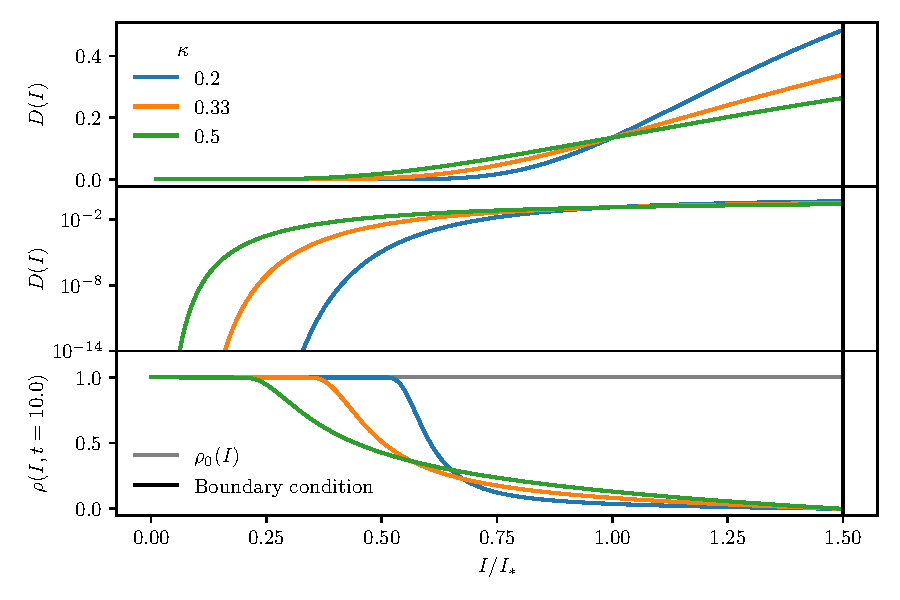
\includegraphics[width=\textwidth]{4_probing_the_diffusive_behavior/figs/diffusion_coefficient.pdf}
    \caption{Top and centre: plot of $D(I)$ both in linear and logarithmic scale for three values of $\kappa$ as a function of $I/I_\ast$.
    %For the cases shown here, the choice $c=1$ has been made, to have comparable curves.
    Bottom: evolution of an uniform distribution (in grey) over the same time interval corresponding to $(t=10.0 \, [\text{a. u.}])$ for three values of $\kappa$. (Simulations parameter: $(I_\ast = 1.0\,[\sigma^2])$).}
    \label{fig:1}
\end{figure*}

